%this file is the first report
%a % comment anything after % until the end of the line

%minimum references to begin our article
\documentclass[12pt]{article}
\usepackage[frenchb]{babel}
\usepackage[utf8]{inputenc}
\usepackage[T1]{fontenc}
\usepackage{graphicx}
\usepackage{fancyhdr}
\usepackage{hyperref}
\usepackage{float}
\usepackage{amsmath}
\usepackage[margin=1in]{geometry}
\usepackage{indentfirst}
\usepackage[section]{placeins}
\usepackage{titlesec}


\pagestyle{fancy}
%\cfoot{Insattack : Projet de POO}
% the last extension makes it possible to add images

%presentation of the document
\title{Insattack : Projet de POO\smallbreak Rapport de conception}
\author{Baptiste \textsc{Bignon}, Gabriel \textsc{Prevosto}}
\date{12/11/2014}
\setlength\parindent{15pt}
\begin{document}

\maketitle
\vfill %tous les vfill prennent la même place

\begin{figure}[!h]
\centering

\includegraphics[width=\textwidth]{Parties/Images/Logo}
\label{fig:logo}
\end{figure}

\vfill
\vfill
\newpage

%to add a table of contents
\tableofcontents
\renewcommand{\contentsname}{Sommaire}
\newpage


\section{Introduction}			\label{sec:introduction}			
\newpage

\section{Le jeu}				\label{sec:jeu}
\subsection{Les règles}			\label{sec:regles}				\subsubsection{Principe du jeu}
INSAttack est un jeu à deux joueurs au tour par tour, chaque joueur choisit son département parmi : INFO, EII, SRC, SGM, GMA, GC. En fonction de son choix ses unités disposeront de différentes capacités (voir partie\ref{sec:departements}). Au début du jeu, les unités de chaque joueur sont rassemblés sur sa case de départ. Afin de gagner la partie un joueur doit éliminer toutes les unités adverses ou avoir un maximum de points à la fin du nombre de tours imparti. Pour cela chaque case qu'il posséde une lui rapporte 2 point. Certains départements peuvent aussi gagner des points grâce à leurs capacités, ou gagner plus ou moins de points selon les types de cases contrôlés.

\subsubsection{Les déplacements}
Pour déplacer une unité, il faut faire un clic gauche sur la case la contenant, puis sur l'unité voulue dans la liste qui s'affichera sur la gauche. Une fois cela fait vous pouvez la déplacer sur une case en faisant un clic droit dessus. L'unité se déplacera si le mouvement est possible, c'est à dire si elle posséde suffisament de points de déplacement et si la case est adjacente.

\subsubsection{Les combats}
Vous pouvez bien sûr attaquer les unités adverses simplement en déplaçant l'une de vos unités sur la case où se trouve votre cible. Le combat sera alors déclenché, un nombre de tour sera choisi aléatoirement, durant chacun d'entre eux les chances de gagner de l'attaquant seront calculées en fonction de son attaque et de la défense de son adversaire. L'unité qui perd un tour de combat perd 1 point de vie. Le combat se termine si l'une des unités meurt ou que tous les tours ont été réalisés. Si l'unité ciblée est morte l'attaquant se déplace sur la case qu'elle occupait. Quelle soit réussie ou non, une attaque consomme autant de points de déplacement qu'un mouvement vers cette case.
\subsection{Les peuples}			\label{sec:départements}				il existe six départements jouables cependant seuls trois d'entre eux disposent de capacités spéciales. 

\subsubsection{Les Info}
\begin{itemize}
\item Le coût de déplacement est augmenté de multiplié par 1.5 sur les cases extérieures.
\item Le coût de déplacement depuis les salles infos est divisé par 2.
\item Les unités de ce département peuvent se téléporter sans utiliser de points de points de déplacement sur n'importe quelle salle info qui n'est pas occupée par des unités adverses.
\end{itemize}

\subsubsection{Les EII}
\begin{itemize}
\item Le coût de déplacement depuis les amphitheâtres est multiplié par 2.
\item Le coût de déplacement depuis les salles de td est divisé par 2.
\item Les unités de ce département gagent 1 point bonus à chaque fois qu'elles tuent un ennemi. Ces points sont liés à l'unité et donc perdus si elle meurt.
\end{itemize} 

\subsubsection{Les SRC}
\begin{itemize}
\item Le coût de déplacement depuis les salles infos est multiplié par 2.
\item Le coût de déplacement depuis les cases extérieures est divisé par 2.
\item Les unités de ce département ont 50\% de chance de fuir un combat perdu et d'échapper à la mort en conservant 1 point de vie. 
\end{itemize}

Les trois autres départements GMA, GC et SGM ont un coût de déplacement de 1 depuis n'importe quelle case et sont dépourvues de la moindre capacité spéciale.
\subsection{Les terrains}			\label{sec:terrains}				\subsubsection{Les cases}
La carte du monde est constituée de cinq types de cases hexagonales : les salles infos, les salles de TD, les amphitheâtres, le self et les extérieures.
Il y a de un à trois self selon le type de map choisi, la moitié des cases sont des extérieurs, et le reste est réparti équitablement entre les autres types de cases.
\begin{figure}[!h]
\centering
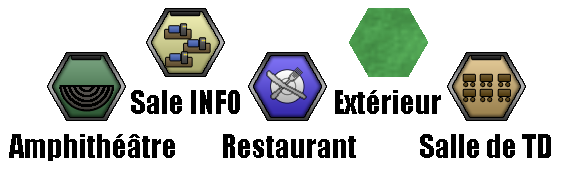
\includegraphics[width=.7\textwidth]{Parties/Images/Terrains.png}
\caption{Les différentes cases, comme elles sont représentées dans le jeu}
\label{fig:Terrains}
\end{figure}

\subsubsection{Les différents types de jeu}
Il existe trois cartes différentes :
\begin{itemize}
\item Démo : 2 joueurs, 6*6 cases, 5 tours, 4 unités par joueur.
\item Petite : 2 joueurs, 10*10 cases, 20 tours, 6 unités par joueur.
\item Démo : 2 joueurs, 14*14 cases, 30 tours, 8 unités par joueur.
\end{itemize}
\clearpage


\clearpage

\section{Conclusion} 			\label{sec:conclusion}			


\end{document}
